\chapter{Pola Desain Perilaku 1}



\section{Pendahuluan}
Pola desain perilaku (\textit{behavioral design patterns}) merupakan pendekatan pemrograman berorientasi objek yang fokus pada bagaimana objek saling berinteraksi dan bertukar tanggung jawab secara dinamis. Bab ini membahas empat pola penting—\textit{Interpreter}, \textit{Observer}, \textit{Strategy}, dan \textit{Command}—yang masing-masing dirancang untuk menangani kebutuhan yang berbeda, mulai dari interpretasi ekspresi, penyebaran notifikasi antar objek, pemilihan algoritma yang dapat diganti saat runtime, hingga pembungkusan aksi sebagai objek. Pemahaman pola-pola ini akan membantu pengembang membangun sistem yang modular, fleksibel, dan mudah dipelihara.


\section{Interpreter}

\subsection{Tujuan dan Konteks Penggunaan}

Pola \textit{Interpreter} adalah pola desain perilaku yang digunakan untuk mendefinisikan representasi gramatika bahasa dan menyediakan cara untuk menginterpretasikan kalimat dalam bahasa tersebut. Pola ini sangat berguna dalam sistem yang memerlukan parsing dan evaluasi terhadap struktur ekspresi berulang, seperti ekspresi matematika, kueri sederhana, atau bahasa domain khusus (DSL - Domain Specific Language).

Tujuan utama dari pola Interpreter adalah untuk:
\begin{itemize}
	\item Mendefinisikan tata bahasa (grammar) dan representasi internal dari suatu bahasa atau ekspresi.
	\item Memberikan antarmuka interpretasi (evaluation) terhadap ekspresi tersebut.
	\item Memisahkan logika interpretasi dari struktur data, dengan pendekatan rekursif berbasis pohon.
\end{itemize}

Struktur pola Interpreter biasanya terdiri dari:
\begin{itemize}
	\item \textbf{AbstractExpression:} Antarmuka atau kelas abstrak yang mendefinisikan metode interpretasi.
	\item \textbf{TerminalExpression:} Mewakili simbol terminal dalam grammar, seperti angka atau variabel.
	\item \textbf{NonTerminalExpression:} Mewakili ekspresi yang terdiri dari satu atau lebih ekspresi lainnya (misalnya ekspresi aritmatika).
	\item \textbf{Context:} Menyimpan informasi global atau lingkungan yang dibutuhkan saat interpretasi.
\end{itemize}

Pola ini cocok digunakan ketika:
\begin{itemize}
	\item Struktur grammar sederhana dan stabil.
	\item Sistem membutuhkan kemampuan interpretasi langsung terhadap input teks atau struktur ekspresi.
	\item Ingin menyediakan antarmuka evaluasi untuk ekspresi berbasis pohon.
\end{itemize}

Beberapa domain aplikasi umum untuk pola Interpreter antara lain:
\begin{itemize}
	\item Mesin ekspresi aritmatika sederhana (calculator).
	\item Sistem pencarian berbasis ekspresi logika (\texttt{AND}, \texttt{OR}, \texttt{NOT}).
	\item Evaluasi query terhadap data (misalnya query mini terhadap koleksi objek).
	\item Penerapan bahasa skrip atau DSL sederhana.
\end{itemize}

Pola ini memperjelas struktur grammar dan membuat implementasi interpreter modular dan mudah diperluas. Namun, pola ini kurang cocok untuk grammar kompleks karena dapat menghasilkan hirarki kelas yang sangat dalam dan sulit dipelihara.


\subsection{Contoh Kasus Penggunaan}

Pola \textit{Interpreter} digunakan secara luas dalam berbagai skenario yang melibatkan evaluasi ekspresi, pemrosesan aturan, atau interpretasi struktur bahasa mini. Penggunaannya sangat sesuai ketika terdapat kebutuhan untuk mengekspresikan aturan dalam bentuk sintaks yang dapat dievaluasi secara fleksibel dan berulang. Berikut adalah beberapa contoh konkret:

\textbf{1. Mesin Ekspresi Aritmatika Sederhana} \\
Salah satu contoh paling umum adalah kalkulator ekspresi aritmatika. Misalnya, ekspresi seperti \texttt{(5 + 3) - 2} dapat direpresentasikan sebagai pohon ekspresi, dan setiap node dalam pohon tersebut diinterpretasikan secara rekursif menggunakan pola Interpreter.

\textbf{2. Pencarian dan Penyaringan Data (Query Filter)} \\
Dalam sistem penyaringan atau pencarian data, pola Interpreter dapat digunakan untuk mengekspresikan kondisi pencarian seperti \texttt{name = 'Alice' AND age > 25}. Setiap kondisi menjadi ekspresi terminal, sedangkan operator logika seperti \texttt{AND}, \texttt{OR}, dan \texttt{NOT} diwakili oleh ekspresi non-terminal.

\textbf{3. Evaluasi Bahasa Domain Khusus (DSL)} \\
Dalam pengembangan DSL (Domain Specific Language), pola Interpreter digunakan untuk memetakan sintaks domain ke dalam struktur evaluasi. Contohnya adalah sistem konfigurasi, alur kerja, atau aturan bisnis seperti \texttt{IF order.total > 500 THEN apply\_discount}.

\textbf{4. Sistem Validasi dan Aturan (Rules Engine)} \\
Sistem yang menerapkan serangkaian aturan atau kebijakan (misalnya, sistem asuransi atau kredit) dapat menggunakan pola Interpreter untuk mengevaluasi aturan berdasarkan data klien. Setiap aturan atau kondisi dapat direpresentasikan sebagai ekspresi yang dapat diinterpretasikan terhadap konteks data.

\textbf{5. Pemrosesan Ekspresi Boolean dalam Game atau AI} \\
Dalam pengembangan game, AI sering memerlukan sistem evaluasi kondisi berbasis logika, misalnya: \texttt{EnemyInRange AND HasAmmo}. Ekspresi ini dapat dibangun dan dievaluasi menggunakan pola Interpreter untuk menentukan keputusan AI.

\textbf{6. Parsing dan Evaluasi Format Bahasa Ringan} \\
Misalnya, evaluasi ekspresi dalam format seperti postfix, prefix, atau ekspresi bahasa konfigurasi seperti JSONPath atau XPath sederhana dapat dibangun menggunakan pola Interpreter, di mana struktur pohon ekspresi dibangun dan diinterpretasikan terhadap data.

Dengan contoh-contoh di atas, pola \textit{Interpreter} terbukti bermanfaat di berbagai bidang mulai dari sistem sederhana hingga sistem evaluasi logika kompleks. Namun, pola ini lebih efektif untuk grammar yang tidak terlalu rumit dan ukuran ekspresi yang tidak terlalu besar.


\subsection{Kelebihan dan Kekurangan}

Pola \textit{Interpreter} menawarkan sejumlah keunggulan dalam hal fleksibilitas dan ekspresivitas dalam merepresentasikan dan mengeksekusi aturan atau ekspresi dalam suatu domain spesifik. Namun, penggunaannya juga memiliki batasan tertentu, terutama dalam hal efisiensi dan skalabilitas.

\textbf{Kelebihan:}
\begin{itemize}
	\item \textbf{Mudah dikembangkan dan diperluas:} Setiap aturan atau ekspresi direpresentasikan sebagai kelas terpisah, sehingga penambahan ekspresi baru cukup dengan menambahkan kelas baru tanpa mengubah struktur yang ada.
	
	\item \textbf{Cocok untuk bahasa domain kecil:} Sangat sesuai digunakan untuk DSL (Domain Specific Language) yang sederhana dan memiliki aturan tetap, seperti bahasa konfigurasi, ekspresi aritmatika, atau aturan logika.
	
	\item \textbf{Struktur ekspresi modular dan komposabel:} Ekspresi dapat dibentuk dari komposisi ekspresi yang lebih kecil secara hierarkis (misalnya pohon ekspresi), memungkinkan evaluasi rekursif yang seragam.
	
	\item \textbf{Memisahkan logika dari data:} Evaluasi ekspresi dapat dilakukan secara terpisah dari struktur data yang mendasari, mendukung prinsip pemisahan tanggung jawab.
	
	\item \textbf{Mudah diimplementasikan dan di-debug:} Untuk grammar kecil, struktur interpretasi sangat eksplisit dan dapat dengan mudah ditelusuri secara manual, sangat berguna dalam sistem edukatif atau prototipe awal.
\end{itemize}

\textbf{Kekurangan:}
\begin{itemize}
	\item \textbf{Kurang efisien untuk grammar besar:} Jika bahasa atau grammar yang ingin ditangani cukup kompleks dan ekspresi sangat banyak, struktur berbasis objek dapat menyebabkan overhead performa dan konsumsi memori yang tinggi.
	
	\item \textbf{Proliferasi kelas:} Setiap simbol atau ekspresi memerlukan satu kelas, sehingga implementasi grammar besar akan menghasilkan banyak kelas kecil yang sulit dikelola.
	
	\item \textbf{Tidak cocok untuk runtime dinamis:} Pola ini lebih cocok untuk grammar statis. Jika aturan berubah-ubah saat runtime, sistem interpreter akan menjadi kurang fleksibel dibanding pendekatan berbasis parser atau rule engine dinamis.
	
	\item \textbf{Debugging dan tracing menjadi kompleks:} Pada struktur ekspresi yang dalam atau rekursif, proses debugging bisa sulit karena alur evaluasi tersebar di banyak objek.
	
	\item \textbf{Sulit dioptimasi secara global:} Karena setiap ekspresi berdiri sendiri dan dievaluasi secara lokal, sulit untuk menerapkan optimisasi menyeluruh seperti memoization atau kompilasi ekspresi.
\end{itemize}

Secara keseluruhan, pola \textit{Interpreter} sangat efektif untuk membangun evaluator bahasa kecil atau aturan terstruktur yang dapat diwakili sebagai ekspresi. Namun, untuk grammar yang lebih besar atau sistem dengan kebutuhan performa tinggi, pendekatan lain seperti parser generator, visitor pattern, atau expression evaluator berbasis AST (Abstract Syntax Tree) mungkin lebih tepat.


\subsection{Implementasi dalam Java}

Implementasi pola \textit{Interpreter} dalam Java umumnya melibatkan pembuatan kelas abstrak atau antarmuka untuk ekspresi, serta serangkaian kelas konkret yang mewakili simbol atau operasi dalam grammar. Evaluasi ekspresi dilakukan secara rekursif, di mana setiap ekspresi mengetahui cara mengevaluasi dirinya sendiri berdasarkan konteks yang diberikan.

\begin{figure}[h]
	\centering
	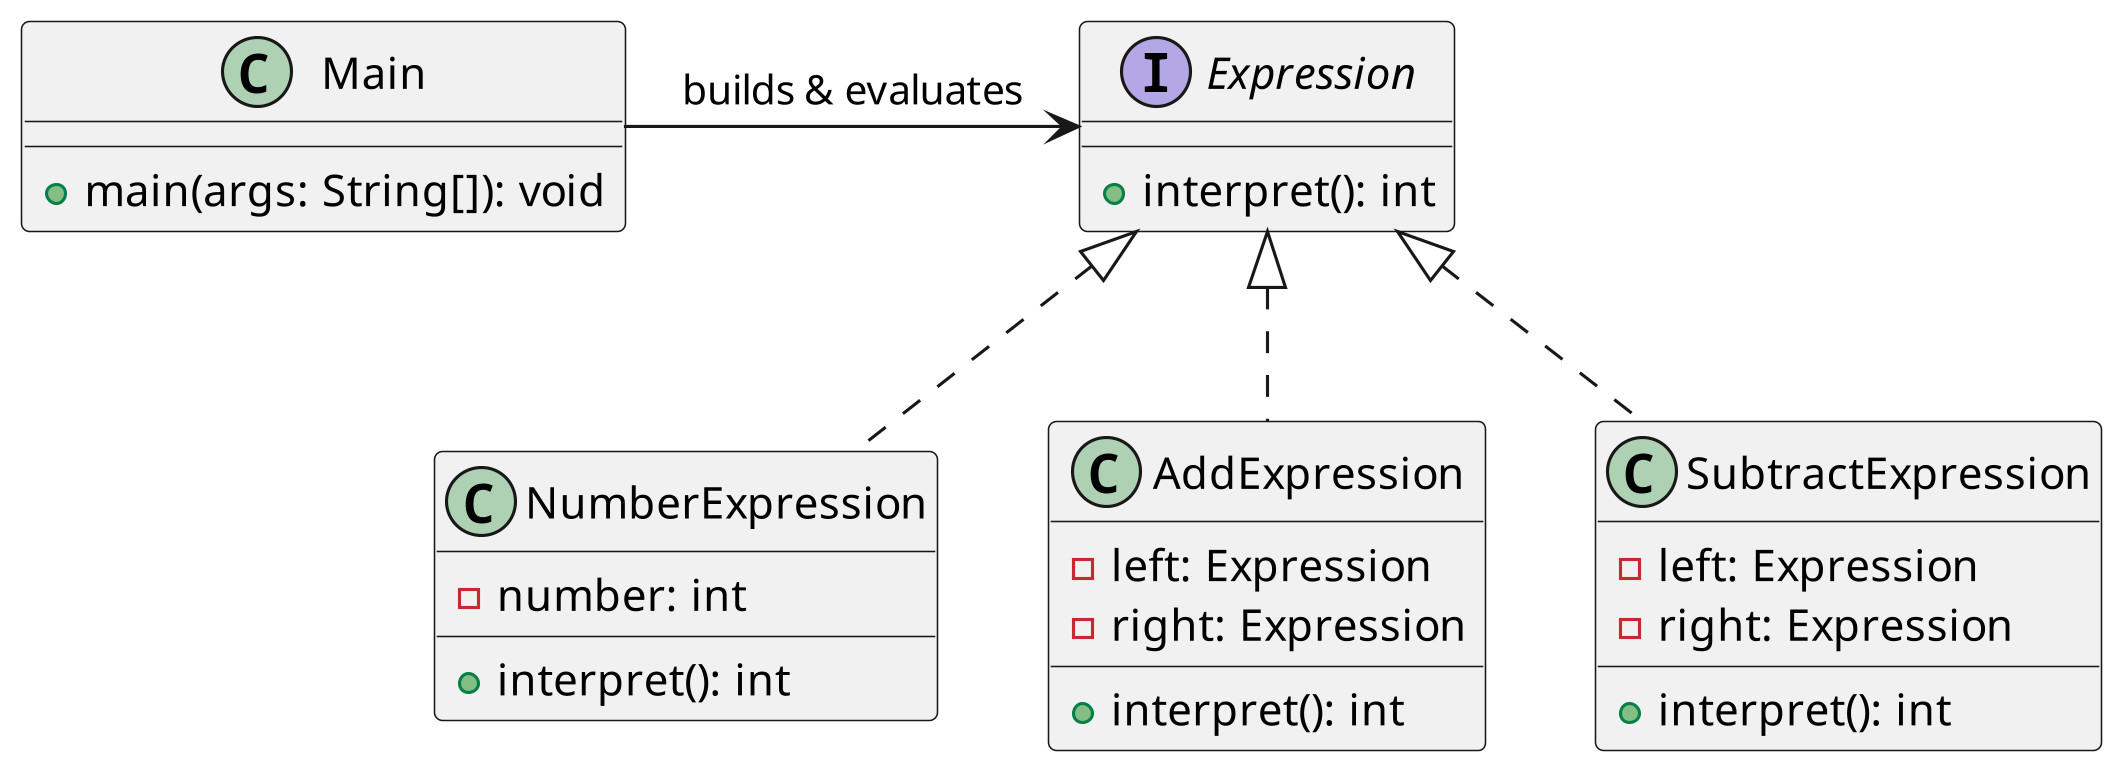
\includegraphics[width=\textwidth]{../figures/out/interpreter.png}
	\caption{Struktur Pola Interpreter}
	\label{fig:interpreter}
\end{figure}


Contoh berikut memperlihatkan penerapan pola \textit{Interpreter} untuk memproses ekspresi aritmatika sederhana dengan operasi penjumlahan dan pengurangan (Gambar \ref{fig:interpreter}).

\begin{lstlisting}[style=JavaStyle, caption={Antarmuka Ekspresi}, label={lst:interpreter-interface}]
	public interface Expression {
		int interpret();
	}
\end{lstlisting}

\begin{lstlisting}[style=JavaStyle, caption={Ekspresi Konstanta (Leaf)}, label={lst:interpreter-number}]
	public class NumberExpression implements Expression {
		private int number;
		
		public NumberExpression(int number) {
			this.number = number;
		}
		
		@Override
		public int interpret() {
			return number;
		}
	}
\end{lstlisting}

\begin{lstlisting}[style=JavaStyle, caption={Ekspresi Penjumlahan}, label={lst:interpreter-plus}]
	public class AddExpression implements Expression {
		private Expression left;
		private Expression right;
		
		public AddExpression(Expression left, Expression right) {
			this.left = left;
			this.right = right;
		}
		
		@Override
		public int interpret() {
			return left.interpret() + right.interpret();
		}
	}
\end{lstlisting}

\begin{lstlisting}[style=JavaStyle, caption={Ekspresi Pengurangan}, label={lst:interpreter-minus}]
	public class SubtractExpression implements Expression {
		private Expression left;
		private Expression right;
		
		public SubtractExpression(Expression left, Expression right) {
			this.left = left;
			this.right = right;
		}
		
		@Override
		public int interpret() {
			return left.interpret() - right.interpret();
		}
	}
\end{lstlisting}

\begin{lstlisting}[style=JavaStyle, caption={Client: Evaluasi Ekspresi}, label={lst:interpreter-main}]
	public class Main {
		public static void main(String[] args) {
			Expression expr = new AddExpression(
			new NumberExpression(10),
			new SubtractExpression(
			new NumberExpression(5),
			new NumberExpression(2)
			)
			);
			
			System.out.println("Result: " + expr.interpret()); // Output: 13
		}
	}
\end{lstlisting}

Pada contoh di atas:
\begin{itemize}
	\item \texttt{Expression} adalah antarmuka dasar untuk semua jenis ekspresi.
	\item \texttt{NumberExpression} adalah ekspresi terminal (leaf) yang hanya menyimpan nilai numerik.
	\item \texttt{AddExpression} dan \texttt{SubtractExpression} adalah ekspresi non-terminal (komposit) yang membentuk ekspresi kompleks dari dua ekspresi lainnya.
	\item Evaluasi dilakukan dengan memanggil \texttt{interpret()} secara rekursif, menyusun hasil dari anak-anak ekspresi.
\end{itemize}

Pola ini dapat dikembangkan lebih lanjut untuk mendukung ekspresi logika, ekspresi variabel dengan konteks (\texttt{Map<String, Integer> context}), atau ekspresi boolean, tergantung pada kebutuhan bahasa domain yang ingin diinterpretasi. Pendekatan ini cocok untuk membangun evaluator DSL (Domain-Specific Language) kecil dan sistem konfigurasi ekspresif.


\section{Observer}

\subsection{Tujuan dan Konteks Penggunaan}

Pola \textit{Observer} merupakan salah satu pola perilaku yang dirancang untuk mendefinisikan relasi satu-ke-banyak antara objek, di mana ketika satu objek (disebut \texttt{Subject}) mengalami perubahan status, seluruh objek lain yang bergantung padanya (disebut \texttt{Observer}) akan diberi notifikasi secara otomatis. Tujuan utama dari pola ini adalah untuk memastikan konsistensi antar objek tanpa menciptakan keterikatan (coupling) secara langsung di antara mereka.

Dengan menggunakan pola \textit{Observer}, sistem menjadi lebih fleksibel dalam menangani skenario di mana satu perubahan harus disebarkan ke banyak bagian lain dalam sistem. Pola ini mendukung prinsip \textit{Loose Coupling} karena \texttt{Subject} tidak perlu mengetahui secara spesifik siapa saja observer-nya, cukup dengan mengelola daftar observer dan memanggil metode \texttt{update()} ketika terjadi perubahan.

Pola ini sangat berguna dalam situasi di mana:
\begin{itemize}
	\item Objek data sering berubah dan perlu memberi tahu banyak bagian sistem (misalnya, tampilan antarmuka) setiap kali terjadi perubahan.
	\item Sistem membutuhkan arsitektur berbasis event, di mana komponen dapat bereaksi terhadap perubahan tanpa saling bergantung secara langsung.
	\item Perlu ada pemisahan antara data dan representasi (misalnya dalam pola \textit{Model-View-Controller}).
\end{itemize}

Komponen utama dalam pola \textit{Observer} meliputi:
\begin{enumerate}
	\item \textbf{Subject (Observable)}: Objek inti yang menyimpan data atau status. Menyediakan antarmuka untuk menambah, menghapus, dan memberi notifikasi kepada observer.
	\item \textbf{Observer}: Objek-objek yang ingin diberi tahu saat \texttt{Subject} berubah. Menerapkan antarmuka tertentu dengan metode seperti \texttt{update()}.
	\item \textbf{ConcreteSubject dan ConcreteObserver}: Implementasi spesifik dari subject dan observer yang berisi logika bisnis masing-masing.
\end{enumerate}

Pola \textit{Observer} secara luas digunakan dalam berbagai sistem, termasuk:
\begin{itemize}
	\item Aplikasi GUI (misalnya, Swing atau JavaFX), di mana perubahan pada model data perlu memperbarui elemen UI secara otomatis.
	\item Sistem event handling atau sistem messaging.
	\item Arsitektur publish-subscribe, di mana klien dapat mendaftar pada topik tertentu dan menerima notifikasi saat event terjadi.
\end{itemize}

Dengan menerapkan pola \textit{Observer}, sistem menjadi lebih modular, dapat dikembangkan secara independen, dan mudah diadaptasi untuk berbagai kebutuhan reaktivitas antar komponen.

\subsection{Contoh Kasus Penggunaan}

Pola \textit{Observer} banyak digunakan dalam sistem perangkat lunak yang membutuhkan mekanisme notifikasi otomatis ketika terjadi perubahan status pada suatu objek. Berikut adalah beberapa contoh kasus penggunaan nyata di berbagai domain:

\textbf{1. Antarmuka Pengguna (User Interface):}  
Dalam aplikasi desktop atau mobile, pola \textit{Observer} digunakan untuk memastikan bahwa komponen tampilan (View) selalu konsisten dengan model data. Ketika data diubah, tampilan yang terdaftar sebagai observer akan diperbarui secara otomatis. Misalnya, dalam arsitektur Model-View-Controller (MVC), komponen View menjadi observer terhadap perubahan dalam Model.

\textbf{2. Sistem Event Handling:}  
Sistem seperti Java AWT/Swing, atau event bus pada framework modern, mengandalkan pola ini untuk mengatur komunikasi antara objek. Misalnya, tombol (\texttt{Button}) sebagai \texttt{Subject} akan memberi tahu listener (\texttt{Observer}) ketika diklik. Dengan demikian, berbagai komponen dapat merespons aksi pengguna secara dinamis tanpa saling bergantung.

\textbf{3. Sinkronisasi Data Antarkomponen:}  
Dalam aplikasi spreadsheet atau grafis, ketika satu sel atau objek diubah, seluruh komponen terkait (misalnya grafik atau hasil perhitungan lain) perlu diperbarui. Pola \textit{Observer} memungkinkan penyebaran perubahan ini secara otomatis tanpa menghubungkan komponen secara langsung.

\textbf{4. Sistem Notifikasi:}  
Aplikasi berita, media sosial, dan platform komunikasi menggunakan pola ini untuk memberi tahu pengguna saat ada konten baru. Misalnya, pengguna yang mengikuti topik atau akun tertentu akan menerima notifikasi saat topik tersebut diperbarui. Di balik layar, topik berperan sebagai \texttt{Subject}, dan pengguna sebagai \texttt{Observer}.

\textbf{5. Sistem Monitoring dan Logging:}  
Dalam sistem server atau aplikasi terdistribusi, modul pemantauan dapat bertindak sebagai observer terhadap status komponen sistem. Jika suatu komponen gagal, observer akan mencatat log, mengirim email, atau memicu alur pemulihan secara otomatis.

\textbf{6. Pasar Keuangan dan Data Feed:}  
Aplikasi perdagangan saham atau crypto biasanya membutuhkan data pasar real-time. Modul antarmuka pasar bertindak sebagai \texttt{Subject}, dan berbagai modul seperti tampilan harga, strategi trading, dan notifikasi akan mendaftar sebagai observer untuk menerima update harga terbaru.

Pola \textit{Observer} sangat bermanfaat ketika dibutuhkan penyebaran perubahan ke banyak bagian sistem secara otomatis, tanpa mengikat implementasi secara langsung. Pendekatan ini meningkatkan skalabilitas dan keterpisahan logika antar komponen.

\subsection{Kelebihan dan Kekurangan}

Pola \textit{Observer} menawarkan mekanisme yang efektif untuk mengatur komunikasi satu-ke-banyak antara objek-objek dalam sistem. Namun, seperti semua pola desain, penerapannya memiliki kelebihan dan kekurangan yang perlu dipertimbangkan secara cermat sesuai konteks penggunaannya.

\textbf{Kelebihan:}
\begin{itemize}
	\item \textbf{Dekopling antara Subject dan Observer:} Subjek tidak perlu mengetahui detail implementasi observer; hanya perlu tahu bahwa mereka mengikuti antarmuka tertentu. Ini meningkatkan modularitas dan fleksibilitas sistem.
	
	\item \textbf{Mendukung mekanisme notifikasi otomatis:} Perubahan pada satu objek secara otomatis disebarkan ke semua observer, sehingga data dan tampilan selalu sinkron tanpa perlu intervensi manual.
	
	\item \textbf{Mudah diperluas:} Observer baru dapat ditambahkan kapan saja tanpa memodifikasi kode dari subjek. Hal ini sejalan dengan prinsip Open/Closed.
	
	\item \textbf{Meningkatkan reaktivitas sistem:} Cocok untuk sistem real-time dan event-driven di mana banyak bagian perlu merespons satu peristiwa yang sama.
	
	\item \textbf{Penerapan yang luas dan terstandarisasi:} Telah didukung secara native di banyak bahasa dan framework, seperti Java (\texttt{Observer/Observable}) dan C\# (event dan delegate).
\end{itemize}

\textbf{Kekurangan:}
\begin{itemize}
	\item \textbf{Sulit ditelusuri dan diuji:} Karena efek samping dari notifikasi tersebar ke banyak observer, jejak eksekusi bisa menjadi kompleks dan sulit ditelusuri saat debugging.
	
	\item \textbf{Potensi masalah kinerja:} Jika jumlah observer sangat banyak atau logika update terlalu berat, notifikasi dapat menyebabkan penurunan performa.
	
	\item \textbf{Keterkaitan implisit:} Meskipun secara teknis terpisah, ada ketergantungan implisit antara subjek dan observer yang bisa menyebabkan dampak tak terduga jika tidak dikelola dengan baik.
	
	\item \textbf{Masalah memori (memory leaks):} Jika observer tidak dihapus secara eksplisit dari daftar observer subjek, maka objek bisa terus berada dalam memori (terutama dalam bahasa tanpa garbage collection otomatis terhadap referensi terdaftar).
	
	\item \textbf{Urutan notifikasi tidak terjamin:} Observer biasanya diberi tahu tanpa urutan yang pasti, yang bisa menjadi masalah jika ada ketergantungan antar observer dalam pengolahan data.
\end{itemize}

Secara keseluruhan, pola \textit{Observer} sangat berguna untuk membangun sistem yang reaktif, modular, dan mudah diperluas. Namun, harus digunakan dengan kehati-hatian dalam sistem besar dan kompleks untuk menghindari masalah skalabilitas dan pemeliharaan.


\subsection{Implementasi dalam Java}

Implementasi pola \textit{Observer} dalam Java dapat dilakukan dengan dua pendekatan utama: menggunakan antarmuka buatan sendiri atau menggunakan API standar Java. Sejak Java 9, kelas bawaan \texttt{Observable} telah dinyatakan deprecated, sehingga pendekatan berbasis antarmuka lebih disarankan untuk fleksibilitas dan pemahaman konsep yang lebih dalam.


\begin{figure}[h]
	\centering
	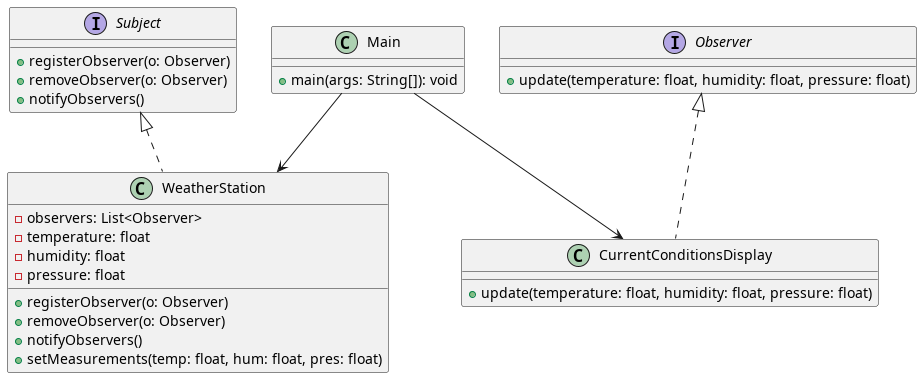
\includegraphics[width=\textwidth]{../figures/out/observer.png}
	\caption{Struktur Pola Observer}
	\label{fig:observer}
\end{figure}

Contoh berikut menunjukkan cara mengimplementasikan pola \textit{Observer} secara manual dengan mendefinisikan antarmuka \texttt{Observer} dan \texttt{Subject}, serta kelas \texttt{WeatherStation} sebagai subjek dan beberapa kelas \texttt{Display} sebagai observer (Gambar \ref{fig:observer}).

\begin{lstlisting}[style=JavaStyle, caption={Antarmuka Subject dan Observer}]
	public interface Observer {
		void update(float temperature, float humidity, float pressure);
	}
	
	public interface Subject {
		void registerObserver(Observer o);
		void removeObserver(Observer o);
		void notifyObservers();
	}
\end{lstlisting}

\begin{lstlisting}[style=JavaStyle, caption={Kelas WeatherStation sebagai Subject}]
	import java.util.*;
	
	public class WeatherStation implements Subject {
		private List<Observer> observers = new ArrayList<>();
		private float temperature, humidity, pressure;
		
		@Override
		public void registerObserver(Observer o) {
			observers.add(o);
		}
		
		@Override
		public void removeObserver(Observer o) {
			observers.remove(o);
		}
		
		@Override
		public void notifyObservers() {
			for (Observer o : observers) {
				o.update(temperature, humidity, pressure);
			}
		}
		
		public void setMeasurements(float temp, float hum, float pres) {
			this.temperature = temp;
			this.humidity = hum;
			this.pressure = pres;
			notifyObservers();
		}
	}
\end{lstlisting}

\begin{lstlisting}[style=JavaStyle, caption={Observer: CurrentConditionsDisplay}]
	public class CurrentConditionsDisplay implements Observer {
		@Override
		public void update(float temperature, float humidity, float pressure) {
			System.out.println("Current Conditions: " + temperature 
			+ " C, " + humidity + "% humidity, " + pressure + " hPa");
		}
	}
\end{lstlisting}

\begin{lstlisting}[style=JavaStyle, caption={Client: Main}]
	public class Main {
		public static void main(String[] args) {
			WeatherStation station = new WeatherStation();
			Observer display = new CurrentConditionsDisplay();
			
			station.registerObserver(display);
			station.setMeasurements(26.5f, 65f, 1012f);
		}
	}
\end{lstlisting}

Pada contoh di atas:
\begin{itemize}
	\item \texttt{WeatherStation} adalah kelas yang berperan sebagai \texttt{Subject} dan menyimpan daftar observer.
	\item \texttt{CurrentConditionsDisplay} adalah salah satu implementasi dari \texttt{Observer} yang bereaksi terhadap perubahan.
	\item Metode \texttt{setMeasurements()} mengubah nilai cuaca dan memberi tahu semua observer secara otomatis.
\end{itemize}

Pendekatan ini menunjukkan kekuatan pola \textit{Observer} dalam menciptakan sistem yang reaktif dan loosely-coupled, memungkinkan klien menambahkan atau menghapus observer tanpa mengubah kode subjek.


\section{Strategy}

\subsection{Tujuan dan Konteks Penggunaan}

Pola \textit{Strategy} adalah pola desain perilaku yang bertujuan untuk memisahkan algoritma dari objek yang menggunakannya, dengan mendefinisikan satu keluarga algoritma, membungkus masing-masing algoritma dalam kelas terpisah, dan membuatnya dapat dipertukarkan secara dinamis. Dengan pendekatan ini, pola \textit{Strategy} memungkinkan objek untuk mengubah perilakunya tanpa harus mengubah kode internalnya.

Tujuan utama dari pola ini adalah untuk:
\begin{itemize}
	\item Menghindari pengulangan kode dan struktur kondisional yang kompleks seperti \texttt{if-else} atau \texttt{switch-case}.
	\item Meningkatkan fleksibilitas dengan memungkinkan pemilihan algoritma yang tepat pada waktu eksekusi.
	\item Memisahkan tanggung jawab antara objek utama dan logika algoritma yang dapat berubah-ubah.
\end{itemize}

Struktur utama dari pola \textit{Strategy} terdiri dari:
\begin{itemize}
	\item \textbf{Strategy (Interface):} Mendefinisikan antarmuka umum untuk semua algoritma atau perilaku.
	\item \textbf{ConcreteStrategy:} Implementasi spesifik dari strategi atau algoritma.
	\item \textbf{Context:} Objek yang menggunakan strategi tertentu dan menyediakan antarmuka kepada klien. Objek ini dapat mengatur strategi secara dinamis.
\end{itemize}

Pola \textit{Strategy} sangat cocok digunakan dalam situasi berikut:
\begin{itemize}
	\item Terdapat banyak algoritma atau variasi logika yang serupa, dan ingin dikelola secara bersih dan modular.
	\item Ingin mengikuti prinsip \textit{Open/Closed} — terbuka untuk ekstensi tetapi tertutup untuk modifikasi.
	\item Perubahan atau penambahan perilaku algoritmik perlu dilakukan tanpa mengubah kelas utama atau klien.
\end{itemize}

Pola ini banyak digunakan dalam sistem yang membutuhkan fleksibilitas perilaku, seperti sistem pembayaran (berbagai metode pembayaran), kompresi file (berbagai algoritma kompresi), atau perhitungan biaya pengiriman (berbagai strategi penghitungan tarif). Dengan memisahkan setiap perilaku ke dalam strategi tersendiri, sistem menjadi lebih mudah dikembangkan, diuji, dan dipelihara.

\subsection{Contoh Kasus Penggunaan}

Pola \textit{Strategy} digunakan dalam berbagai konteks di mana terdapat beberapa cara untuk melakukan suatu tugas atau algoritma, dan pemilihan strategi dilakukan secara dinamis berdasarkan kondisi atau kebutuhan klien. Dengan memisahkan algoritma ke dalam kelas-kelas terpisah, pola ini membuat kode lebih modular, mudah diperluas, dan mudah diuji. Berikut beberapa contoh konkret penggunaannya:

\textbf{1. Sistem Pembayaran Online} \\
Dalam aplikasi e-commerce, pengguna bisa memilih berbagai metode pembayaran seperti kartu kredit, e-wallet, atau transfer bank. Setiap metode memiliki logika pemrosesan yang berbeda. Dengan pola \textit{Strategy}, sistem dapat mengenkapsulasi setiap metode pembayaran dalam kelas strategi yang berbeda, sehingga pemilihan metode pembayaran bisa dilakukan tanpa mengubah logika utama transaksi.

\textbf{2. Algoritma Kompresi File} \\
Aplikasi yang mendukung berbagai algoritma kompresi seperti ZIP, RAR, atau 7z dapat menggunakan pola \textit{Strategy} untuk mengabstraksi proses kompresi. Kelas utama tinggal memilih strategi kompresi yang sesuai berdasarkan preferensi pengguna atau jenis file.

\textbf{3. Perhitungan Tarif Pengiriman} \\
Layanan logistik atau e-commerce sering kali memiliki berbagai cara menghitung tarif pengiriman, seperti tarif berdasarkan berat, volume, atau jarak. Dengan pola \textit{Strategy}, setiap metode perhitungan tarif dapat diimplementasikan sebagai strategi yang dapat dipilih dan digunakan sesuai dengan jenis layanan pengiriman.

\textbf{4. Sorting atau Pencarian dengan Kriteria Berbeda} \\
Dalam sistem manajemen data, pengguna bisa memilih untuk mengurutkan data berdasarkan nama, tanggal, atau prioritas. Masing-masing strategi pengurutan dapat diimplementasikan dalam kelas berbeda, dan digunakan secara dinamis oleh komponen yang membutuhkan.

\textbf{5. Game AI dengan Strategi Berbeda} \\
Dalam permainan seperti catur atau strategi waktu nyata (RTS), pola \textit{Strategy} digunakan untuk mengatur perilaku AI seperti menyerang, bertahan, atau mencari sumber daya. Masing-masing strategi dapat diterapkan sesuai dengan kondisi permainan yang sedang berlangsung.

\textbf{6. Sistem Promosi atau Diskon} \\
Sistem penjualan atau kasir dapat menawarkan diskon dengan berbagai strategi seperti diskon persentase, diskon tetap, atau beli satu gratis satu. Dengan pola \textit{Strategy}, setiap jenis diskon dapat dikemas sebagai strategi yang dapat dipilih dan diterapkan terhadap total belanja.

Dengan contoh-contoh di atas, pola \textit{Strategy} menunjukkan fleksibilitas dan kekuatannya dalam mengorganisir berbagai pilihan perilaku atau algoritma tanpa mencemari logika utama aplikasi. Pendekatan ini mendukung sistem yang mudah dikembangkan dan disesuaikan untuk kebutuhan masa depan.

\subsection{Kelebihan dan Kekurangan}

Pola \textit{Strategy} memberikan solusi elegan terhadap permasalahan variasi perilaku atau algoritma dalam aplikasi dengan cara mendekompisisikannya ke dalam kelas-kelas terpisah yang dapat dipertukarkan. Meski fleksibel, pola ini juga memiliki beberapa keterbatasan yang perlu diperhatikan.

\textbf{Kelebihan:}
\begin{itemize}
	\item \textbf{Memisahkan perilaku dari konteks:} Strategi mengisolasi algoritma atau logika tertentu dari kelas utama, sehingga kelas utama menjadi lebih bersih dan fokus pada tanggung jawab utamanya.
	
	\item \textbf{Mendukung prinsip Open/Closed:} Kode terbuka untuk ekstensi tetapi tertutup untuk modifikasi. Artinya, strategi baru dapat ditambahkan tanpa harus mengubah kode yang sudah ada.
	
	\item \textbf{Mengurangi duplikasi kode:} Dengan mengenkapsulasi algoritma dalam kelas terpisah, pola ini mencegah duplikasi logika yang sama di banyak tempat.
	
	\item \textbf{Meningkatkan fleksibilitas:} Perilaku dapat diganti selama runtime, misalnya dalam program interaktif atau sistem konfigurasi dinamis.
	
	\item \textbf{Mendukung unit testing:} Setiap strategi dapat diuji secara terpisah, karena strategi merupakan entitas independen dengan antarmuka eksplisit.
\end{itemize}

\textbf{Kekurangan:}
\begin{itemize}
	\item \textbf{Peningkatan jumlah kelas:} Setiap strategi perlu diimplementasikan dalam kelas terpisah, sehingga dalam kasus dengan banyak algoritma, jumlah kelas bisa bertambah secara signifikan.
	
	\item \textbf{Kompleksitas konfigurasi:} Pengelolaan dan pemilihan strategi yang tepat pada runtime bisa menjadi kompleks, terutama bila strategi melibatkan dependensi tambahan.
	
	\item \textbf{Tidak menjamin pertukaran penuh:} Meskipun strategi memiliki antarmuka yang sama, tidak semua strategi selalu cocok untuk semua konteks. Kesalahan pemilihan strategi dapat menyebabkan perilaku tak diinginkan.
	
	\item \textbf{Overhead tambahan:} Karena strategi dipanggil melalui komposisi objek (delegasi), akan ada overhead tambahan dalam hal pemanggilan fungsi dibandingkan logika langsung.
	
	\item \textbf{Tidak ideal untuk algoritma sederhana:} Untuk algoritma yang sangat kecil atau hanya satu baris, penggunaan pola ini bisa terasa terlalu rumit dan tidak efisien.
\end{itemize}

Secara keseluruhan, pola \textit{Strategy} sangat tepat digunakan ketika sistem perlu mendukung berbagai variasi algoritma atau perilaku yang dapat diganti tanpa menyentuh kode utama. Namun, penggunaannya harus disesuaikan dengan kompleksitas dan kebutuhan sistem untuk menghindari desain yang terlalu abstrak.

\subsection{Implementasi dalam Java}

Implementasi pola \textit{Strategy} dalam Java melibatkan pembuatan antarmuka untuk mendefinisikan perilaku atau algoritma yang dapat diganti-ganti, serta kelas-kelas konkret yang mengimplementasikan strategi tersebut. Objek \texttt{Context} kemudian menggunakan strategi tertentu yang dipilih saat runtime.

Pola ini memungkinkan klien untuk dengan mudah mengganti strategi tanpa mengubah logika utama dalam kelas \texttt{Context}. Pemilihan strategi dapat dilakukan melalui konfigurasi, input pengguna, atau logika internal sistem.

\begin{figure}[h]
	\centering
	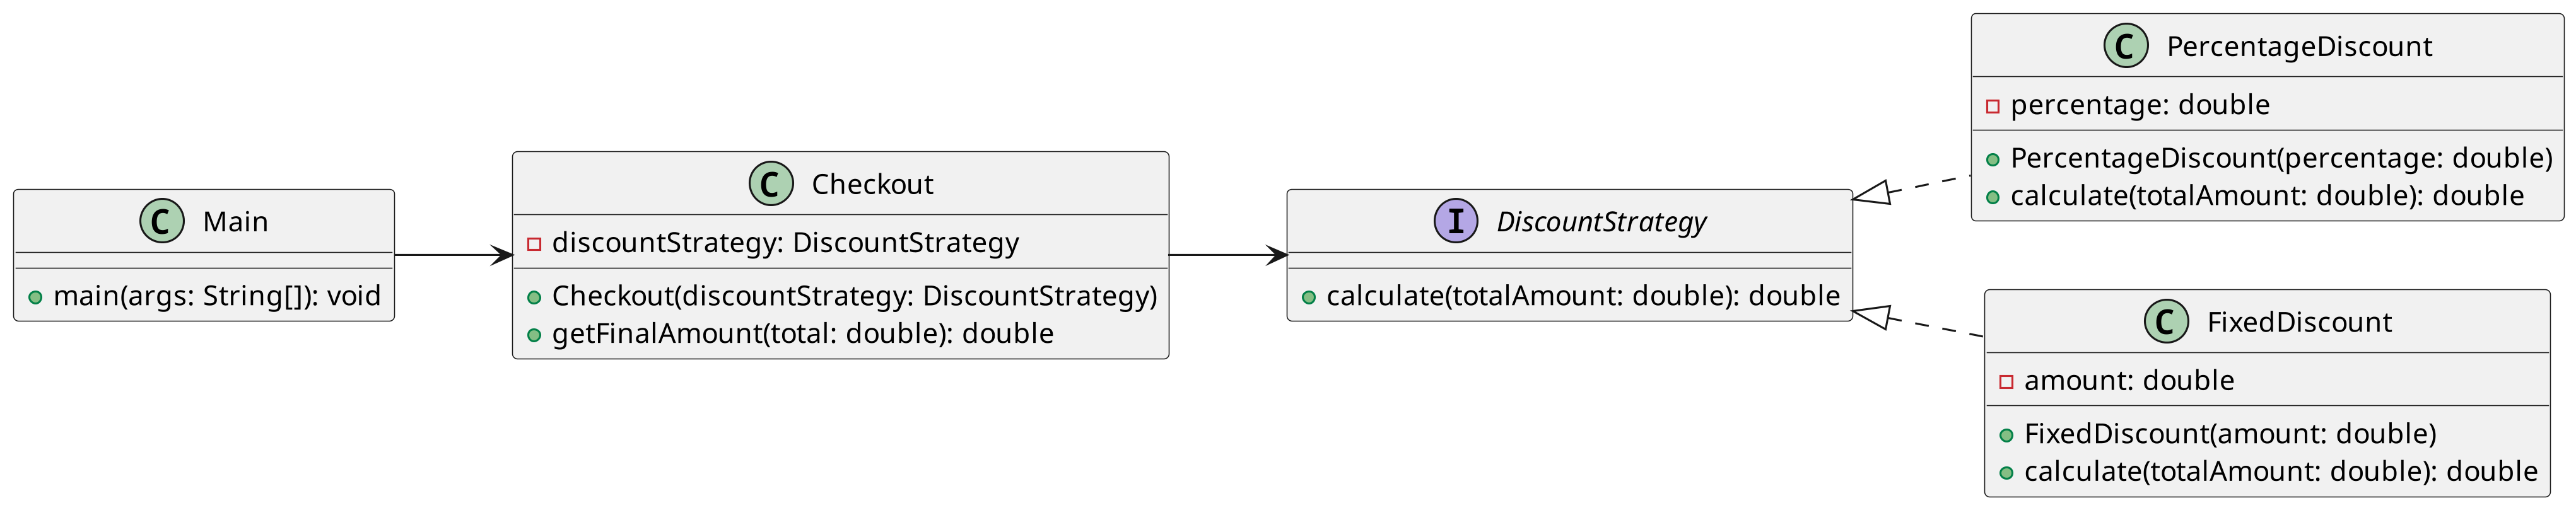
\includegraphics[width=\textwidth]{../figures/out/strategy.png}
	\caption{Struktur Pola Strategy}
	\label{fig:strategy}
\end{figure}

Contoh berikut menunjukkan bagaimana pola \textit{Strategy} diterapkan dalam konteks sistem perhitungan diskon, di mana strategi diskon dapat diganti-ganti (Gambar~\ref{fig:strategy}).

\begin{lstlisting}[style=JavaStyle, caption={Antarmuka Strategy}, label={lst:strategy-interface}]
	public interface DiscountStrategy {
		double calculate(double totalAmount);
	}
\end{lstlisting}

\begin{lstlisting}[style=JavaStyle, caption={Strategi Diskon Persentase}, label={lst:strategy-percentage}]
	public class PercentageDiscount implements DiscountStrategy {
		private double percentage;
		
		public PercentageDiscount(double percentage) {
			this.percentage = percentage;
		}
		
		@Override
		public double calculate(double totalAmount) {
			return totalAmount * (1 - percentage);
		}
	}
\end{lstlisting}

\begin{lstlisting}[style=JavaStyle, caption={Strategi Diskon Tetap}, label={lst:strategy-fixed}]
	public class FixedDiscount implements DiscountStrategy {
		private double amount;
		
		public FixedDiscount(double amount) {
			this.amount = amount;
		}
		
		@Override
		public double calculate(double totalAmount) {
			return totalAmount - amount;
		}
	}
\end{lstlisting}

\begin{lstlisting}[style=JavaStyle, caption={Context: Kasir atau Checkout}, label={lst:strategy-context}]
	public class Checkout {
		private DiscountStrategy discountStrategy;
		
		public Checkout(DiscountStrategy discountStrategy) {
			this.discountStrategy = discountStrategy;
		}
		
		public double getFinalAmount(double total) {
			return discountStrategy.calculate(total);
		}
	}
\end{lstlisting}

\begin{lstlisting}[style=JavaStyle, caption={Client: Menggunakan Strategi Diskon}, label={lst:strategy-client}]
	public class Main {
		public static void main(String[] args) {
			double total = 100.0;
			
			// Menggunakan strategi diskon 20%
			DiscountStrategy percentage = new PercentageDiscount(0.2);
			Checkout checkout1 = new Checkout(percentage);
			System.out.println("Total setelah diskon persentase: " + checkout1.getFinalAmount(total));
			
			// Menggunakan strategi diskon tetap Rp 15
			DiscountStrategy fixed = new FixedDiscount(15.0);
			Checkout checkout2 = new Checkout(fixed);
			System.out.println("Total setelah diskon tetap: " + checkout2.getFinalAmount(total));
		}
	}
\end{lstlisting}

Penjelasan dari implementasi di atas:
\begin{itemize}
	\item \texttt{DiscountStrategy} adalah antarmuka yang mendefinisikan kontrak perhitungan diskon.
	\item \texttt{PercentageDiscount} dan \texttt{FixedDiscount} adalah implementasi dari strategi diskon yang berbeda.
	\item \texttt{Checkout} adalah \texttt{Context} yang menggunakan strategi yang diberikan untuk menghitung harga akhir.
	\item Strategi dapat diganti secara dinamis tergantung kondisi, tanpa harus mengubah kode dalam kelas \texttt{Checkout}.
\end{itemize}

Pendekatan ini sangat cocok untuk sistem yang membutuhkan variasi perilaku seperti sistem promosi, algoritma kompresi, perhitungan ongkir, strategi pergerakan karakter dalam game, dan lain sebagainya.


\section{Command}

\subsection{Tujuan dan Konteks Penggunaan}

Pola \textit{Command} adalah pola desain perilaku yang bertujuan untuk mengenkapsulasi sebuah permintaan (request) sebagai objek, sehingga memungkinkan parameterisasi terhadap klien dengan berbagai permintaan, antrean permintaan, serta kemampuan untuk membatalkan atau mencatat permintaan tersebut. Pola ini memisahkan objek yang mengeluarkan perintah dari objek yang mengeksekusi perintah, dengan cara membungkus perintah tersebut dalam bentuk objek.

Tujuan utama dari pola ini adalah untuk:
\begin{itemize}
	\item Memisahkan pengirim perintah (\texttt{Invoker}) dari penerima perintah (\texttt{Receiver}).
	\item Memungkinkan penyimpanan, log, atau pembatalan perintah (undo/redo).
	\item Mendukung antrean tugas atau makro (sekumpulan perintah).
\end{itemize}

Struktur utama dari pola \textit{Command} melibatkan:
\begin{itemize}
	\item \textbf{Command (Interface):} Mendefinisikan antarmuka umum untuk semua perintah, biasanya dengan metode \texttt{execute()}.
	\item \textbf{ConcreteCommand:} Implementasi spesifik dari perintah, yang menyimpan referensi ke objek \texttt{Receiver} dan memanggil metode yang sesuai.
	\item \textbf{Receiver:} Objek aktual yang berisi logika bisnis untuk mengeksekusi perintah.
	\item \textbf{Invoker:} Objek yang meminta perintah untuk dieksekusi, tanpa mengetahui detail implementasi atau penerima.
	\item \textbf{Client:} Objek yang mengatur hubungan antara perintah, penerima, dan pengirim.
\end{itemize}

Pola ini sangat bermanfaat dalam situasi berikut:
\begin{itemize}
	\item Ketika sistem memerlukan antrean atau penjadwalan tugas.
	\item Untuk mendukung operasi undo/redo atau logging histori aksi.
	\item Ketika banyak jenis permintaan berbeda perlu dipicu secara dinamis.
	\item Untuk membuat sistem makro, di mana beberapa perintah dieksekusi dalam satu langkah.
\end{itemize}

Contoh aplikasi umum dari pola \textit{Command} meliputi:
\begin{itemize}
	\item Sistem GUI: setiap aksi tombol atau menu direpresentasikan sebagai objek \texttt{Command} yang dapat dijalankan, dibatalkan, atau direkam.
	\item Sistem remote control: tombol remote dikaitkan dengan berbagai perintah terhadap perangkat (TV, AC, dll).
	\item Sistem perintah dalam game atau editor teks: mendukung undo, redo, atau makro pengguna.
	\item Arsitektur task queue atau job scheduler.
\end{itemize}

Dengan menerapkan pola ini, sistem memperoleh fleksibilitas tinggi untuk menambahkan, mengelola, dan melacak berbagai jenis perintah tanpa mengubah logika utama pemrosesan.

\subsection{Contoh Kasus Penggunaan}

Pola \textit{Command} digunakan secara luas dalam berbagai sistem perangkat lunak yang memerlukan pemisahan antara pemicu perintah dan eksekutor perintah, serta ketika perintah perlu dicatat, dibatalkan, atau dijalankan ulang. Dengan membungkus aksi sebagai objek, pola ini memberikan fleksibilitas dalam pengelolaan dan orkestrasi perintah. Berikut adalah beberapa contoh nyata penerapannya:

\textbf{1. Aksi Tombol dalam GUI (Graphical User Interface)} \\
Dalam aplikasi desktop seperti editor teks atau pengolah gambar, setiap klik pada tombol seperti \texttt{Save}, \texttt{Copy}, atau \texttt{Undo} dipetakan ke objek \texttt{Command}. Hal ini memungkinkan sistem mencatat urutan perintah pengguna dan mendukung fitur undo/redo.

\textbf{2. Sistem Remote Control} \\
Dalam sistem pengendali jarak jauh (misalnya pengontrol rumah pintar), setiap tombol pada remote dapat dikaitkan dengan objek \texttt{Command} yang mewakili tindakan seperti menyalakan lampu, menutup tirai, atau mengaktifkan AC. Perintah-perintah ini bisa disimpan, dijadwalkan, atau dijalankan secara berurutan (makro).

\textbf{3. Manajemen Perintah dalam Game} \\
Dalam game strategi atau simulasi, setiap aksi pemain (misalnya, \texttt{Move}, \texttt{Attack}, \texttt{Build}) direpresentasikan sebagai objek \texttt{Command}. Ini memungkinkan penyimpanan aksi pemain untuk replay, undo, atau skrip otomatis.

\textbf{4. Fitur Undo/Redo dalam Editor} \\
Pola \textit{Command} sangat cocok untuk mendukung operasi \texttt{Undo} dan \texttt{Redo}. Setiap perubahan terhadap dokumen dibungkus sebagai objek \texttt{Command}, dan sistem menyimpan stack perintah yang telah dijalankan. Ketika pengguna menekan \texttt{Undo}, perintah terakhir dibatalkan dengan memanggil metode \texttt{undo()} yang sesuai.

\textbf{5. Eksekusi Perintah dalam Antrian Tugas (Job Queue)} \\
Dalam sistem batch processing atau job scheduler, setiap tugas dikemas sebagai objek \texttt{Command} dan dimasukkan ke dalam antrean. Scheduler hanya perlu mengeksekusi perintah satu per satu tanpa mengetahui isi atau penerima dari perintah tersebut.

\textbf{6. Orkestrasi Layanan dalam Sistem Terdistribusi} \\
Dalam sistem mikrolayanan, pola ini dapat digunakan untuk mengatur rangkaian tindakan lintas layanan, seperti dalam implementasi \textit{Saga Pattern}, di mana setiap langkah transaksi dikemas sebagai perintah dan bisa dijalankan atau dikompensasi.

\textbf{7. Logging dan Audit Trail} \\
Karena setiap perintah dikemas sebagai objek dengan informasi lengkap, sistem dapat dengan mudah mencatat (log) setiap perintah yang dijalankan beserta parameter-parameternya, sehingga mendukung audit dan pelacakan sistem.

Pola \textit{Command} memberikan pendekatan yang bersih dan fleksibel dalam menangani aksi terprogram, memungkinkan pengendalian penuh atas pelaksanaan perintah, pengurutan, pembatalan, hingga pencatatan histori aktivitas pengguna atau sistem.


\subsection{Kelebihan dan Kekurangan}

Pola \textit{Command} menyediakan cara yang terstruktur untuk mengenkapsulasi permintaan sebagai objek, sehingga memungkinkan fleksibilitas tinggi dalam pengelolaan perintah. Namun, seperti semua pola desain, penerapannya memiliki kelebihan dan kekurangan yang perlu dipertimbangkan berdasarkan konteks sistem yang dikembangkan.

\textbf{Kelebihan:}
\begin{itemize}
	\item \textbf{Pemisahan tanggung jawab (separation of concerns):} Pola ini memisahkan objek pengirim perintah (\texttt{Invoker}) dari objek penerima perintah (\texttt{Receiver}). Hal ini mendukung prinsip \textit{loose coupling} dan meningkatkan modularitas.
	
	\item \textbf{Mendukung undo/redo:} Karena perintah dikemas dalam objek mandiri, sistem dapat menyimpan riwayat perintah yang telah dieksekusi, dan melakukan \texttt{undo()} atau \texttt{redo()} dengan mudah.
	
	\item \textbf{Mudah dikembangkan dan diperluas:} Penambahan jenis perintah baru cukup dengan membuat kelas \texttt{ConcreteCommand} baru tanpa mengubah kode pengirim atau penerima.
	
	\item \textbf{Mendukung makro dan scripting:} Beberapa objek \texttt{Command} dapat digabungkan dalam satu objek makro untuk mengeksekusi rangkaian tindakan secara berurutan.
	
	\item \textbf{Dapat diantrikan atau dijadwalkan:} Karena perintah dikemas sebagai objek, ia dapat dimasukkan ke antrean, diproses secara paralel, atau dijadwalkan untuk eksekusi di masa mendatang (seperti dalam sistem batch atau worker thread).
\end{itemize}

\textbf{Kekurangan:}
\begin{itemize}
	\item \textbf{Proliferasi kelas:} Setiap perintah biasanya memerlukan satu kelas konkret, yang dapat meningkatkan jumlah kelas secara signifikan jika jumlah perintah banyak.
	
	\item \textbf{Overhead implementasi:} Untuk tugas-tugas yang sederhana, menggunakan pola ini dapat terasa berlebihan dan memperumit desain dibandingkan sekadar memanggil metode secara langsung.
	
	\item \textbf{Kebutuhan penyimpanan status tambahan:} Untuk mendukung \texttt{undo()}, kelas \texttt{Command} harus menyimpan status sebelumnya, yang dapat menambah kompleksitas dan konsumsi memori.
	
	\item \textbf{Membutuhkan pemetaan tambahan di klien:} Klien bertanggung jawab untuk mengatur hubungan antara tombol (atau pemicu) dan perintah, sehingga menambah langkah konfigurasi.
	
	\item \textbf{Kesulitan dalam debugging dan tracing:} Karena aksi tersebar dalam objek-objek \texttt{Command} yang terpisah, melacak eksekusi sistem bisa lebih kompleks dibandingkan pendekatan prosedural langsung.
\end{itemize}

Secara keseluruhan, pola \textit{Command} sangat ideal untuk aplikasi yang membutuhkan eksekusi terstruktur atas perintah, terutama jika sistem membutuhkan fitur undo/redo, logging, atau orkestrasi tugas kompleks. Namun, dalam sistem kecil dengan logika perintah yang sederhana, pola ini bisa memperkenalkan kompleksitas yang tidak perlu.


\subsection{Implementasi dalam Java}

Implementasi pola \textit{Command} dalam Java dilakukan dengan cara mendefinisikan antarmuka \texttt{Command} yang merepresentasikan perintah, serta membuat kelas-kelas konkret yang mengimplementasikan aksi spesifik. Setiap perintah menyimpan referensi ke objek \texttt{Receiver}, yaitu objek yang memiliki logika aktual untuk melakukan aksi. Objek \texttt{Invoker} akan menyimpan dan menjalankan perintah tanpa mengetahui detail implementasinya.

\begin{figure}[h]
	\centering
		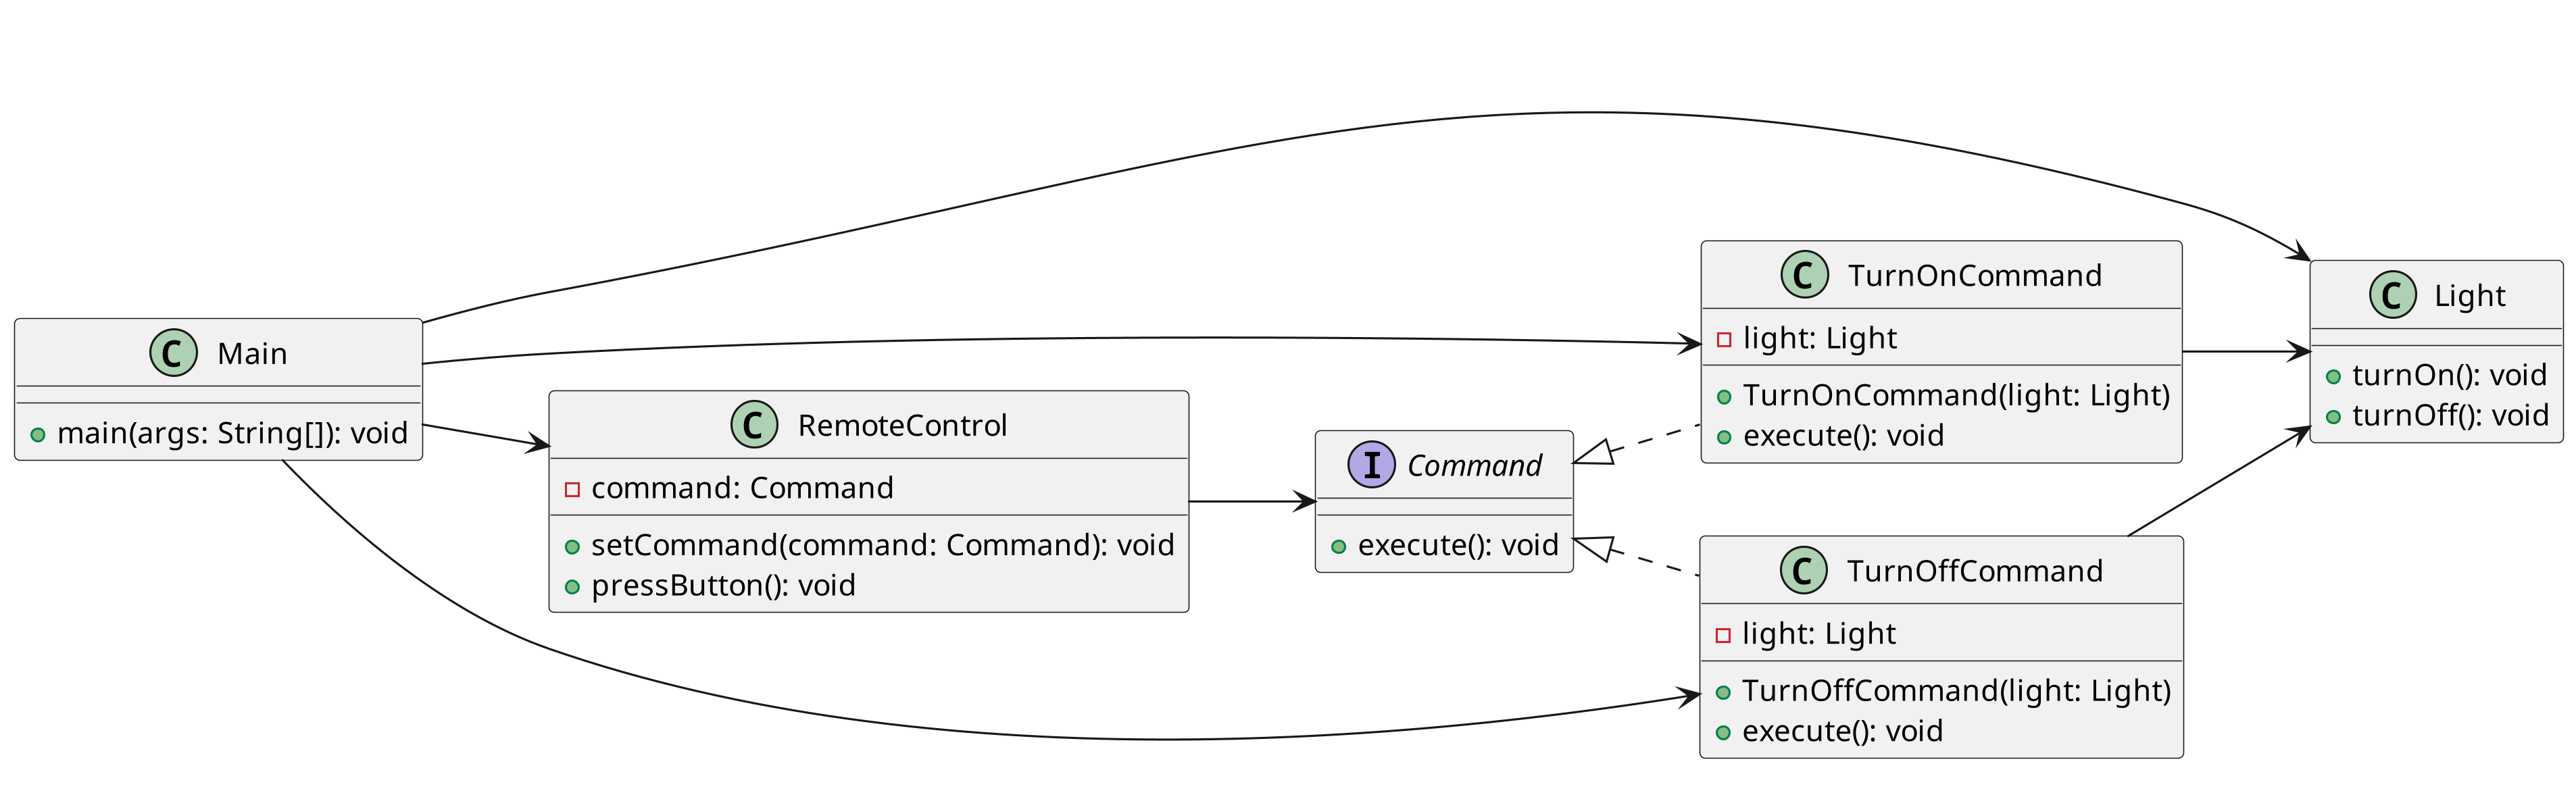
\includegraphics[width=\textwidth]{../figures/out/command.png}
	\caption{Struktur Pola Command}
	\label{fig:command}
\end{figure}

Contoh berikut menunjukkan implementasi pola \textit{Command} dalam sistem kendali perangkat rumah pintar, di mana pengguna dapat menyalakan dan mematikan perangkat seperti lampu.

\begin{lstlisting}[style=JavaStyle, caption={Antarmuka Command}, label={lst:command-interface}]
	public interface Command {
		void execute();
	}
\end{lstlisting}

\begin{lstlisting}[style=JavaStyle, caption={Receiver: Lampu}, label={lst:command-receiver}]
	public class Light {
		public void turnOn() {
			System.out.println("Lampu dinyalakan.");
		}
		
		public void turnOff() {
			System.out.println("Lampu dimatikan.");
		}
	}
\end{lstlisting}

\begin{lstlisting}[style=JavaStyle, caption={ConcreteCommand: Perintah Menyalakan Lampu}, label={lst:command-on}]
	public class TurnOnCommand implements Command {
		private Light light;
		
		public TurnOnCommand(Light light) {
			this.light = light;
		}
		
		@Override
		public void execute() {
			light.turnOn();
		}
	}
\end{lstlisting}

\begin{lstlisting}[style=JavaStyle, caption={ConcreteCommand: Perintah Mematikan Lampu}, label={lst:command-off}]
	public class TurnOffCommand implements Command {
		private Light light;
		
		public TurnOffCommand(Light light) {
			this.light = light;
		}
		
		@Override
		public void execute() {
			light.turnOff();
		}
	}
\end{lstlisting}

\begin{lstlisting}[style=JavaStyle, caption={Invoker: Remote Control}, label={lst:command-invoker}]
	public class RemoteControl {
		private Command command;
		
		public void setCommand(Command command) {
			this.command = command;
		}
		
		public void pressButton() {
			command.execute();
		}
	}
\end{lstlisting}

\begin{lstlisting}[style=JavaStyle, caption={Client: Penggunaan Command}, label={lst:command-client}]
	public class Main {
		public static void main(String[] args) {
			Light livingRoomLight = new Light();
			
			Command lightOn = new TurnOnCommand(livingRoomLight);
			Command lightOff = new TurnOffCommand(livingRoomLight);
			
			RemoteControl remote = new RemoteControl();
			
			remote.setCommand(lightOn);
			remote.pressButton(); // Output: Lampu dinyalakan.
			
			remote.setCommand(lightOff);
			remote.pressButton(); // Output: Lampu dimatikan.
		}
	}
\end{lstlisting}

Penjelasan dari struktur implementasi di atas:
\begin{itemize}
	\item \texttt{Command} adalah antarmuka generik yang mendefinisikan metode \texttt{execute()}.
	\item \texttt{Light} bertindak sebagai \texttt{Receiver} yang melakukan logika aktual (menyalakan/mematikan lampu).
	\item \texttt{TurnOnCommand} dan \texttt{TurnOffCommand} adalah implementasi konkret dari perintah yang memanggil aksi pada \texttt{Receiver}.
	\item \texttt{RemoteControl} adalah \texttt{Invoker} yang mengeksekusi perintah yang telah disetel tanpa mengetahui detail implementasinya.
	\item \texttt{Main} sebagai klien, bertanggung jawab untuk mengatur hubungan antara perintah dan penerima, serta menginisialisasi proses.
\end{itemize}

Dengan pola ini, perintah dapat dengan mudah diperluas (misalnya untuk menambah \texttt{DimLightCommand}, \texttt{SetTimerCommand}), disusun dalam antrian, atau ditambahkan ke dalam sistem undo/redo untuk mengelola perilaku interaktif yang kompleks secara fleksibel.




\section{Kesimpulan}

Keempat pola desain perilaku yang dibahas dalam bab ini — \textit{Interpreter}, \textit{Observer}, \textit{Strategy}, dan \textit{Command} — masing-masing menawarkan solusi terhadap jenis masalah perilaku yang berbeda dalam pengembangan perangkat lunak. Pola \textit{Interpreter} digunakan untuk mengevaluasi ekspresi atau bahasa domain dengan struktur gramatika yang stabil. Pola \textit{Observer} memungkinkan penyebaran notifikasi otomatis ke banyak objek saat terjadi perubahan status, mendukung sistem reaktif dan event-driven.

Sementara itu, pola \textit{Strategy} memisahkan algoritma dari konteks penggunaannya agar dapat diganti secara dinamis tanpa mengubah logika inti, sangat berguna dalam sistem dengan banyak variasi perilaku. Pola \textit{Command} membungkus aksi sebagai objek sehingga mendukung fitur undo/redo, penjadwalan, dan pemrosesan terpisah. Pemilihan pola yang tepat akan membantu menciptakan sistem yang modular, fleksibel, dan mudah dipelihara sesuai kebutuhan arsitektural dan fungsional aplikasi.
